In the previous section, we have introduced the ShICA model, a principled
unifying solution to the problems of shared response
modeling and GroupICA. In this section, we first show on synthetic data that ShICA
outperforms other approaches in terms of the trade-off between statistical
accuracy and computation time. Then, on brain imaging data, we show that ShICA
gives more stable decompositions for comparable computation times, more
accurately predicts the data of one subject from the data of other subjects
making it a good candidate to perform transfer learning and yields superior
accuracy on the timesegment matching experiment.

\section{Synthetic experiment}
In the following synthetic experiments, data are generated according to model~\eqref{eq:model} with $p=4$ components and $m=5$ views and mixing matrices are generated by sampling coefficients from a standardized Gaussian.
\subsection{Separation performance}
\label{sec:rotation}
%\pierre{Make sure that algos are always in the same order in legend, and that shica-j and shica ml are together}
Gaussian components are generated from a standardized Gaussian and their noise has standard deviation $\Sigma_i^{\frac12}$ (obtained by sampling from a uniform density between $0$ and $1$) while non-Gaussian components are generated from a Laplace distribution and their noise standard deviations are equal. We study 3 cases where either all components are Gaussian, all components are non-Gaussian or half of the components are Gaussian and half are non-Gaussian. We vary the number of samples $n$ between $10^2$ and $10^5$ and display in Fig~\ref{exp:rotation} the mean Amari distance across subjects as a function of $n$. The experiment is repeated $100$ times using different seeds. We report the median result and error bars  represent the first and last deciles.
\begin{figure}
\centering
  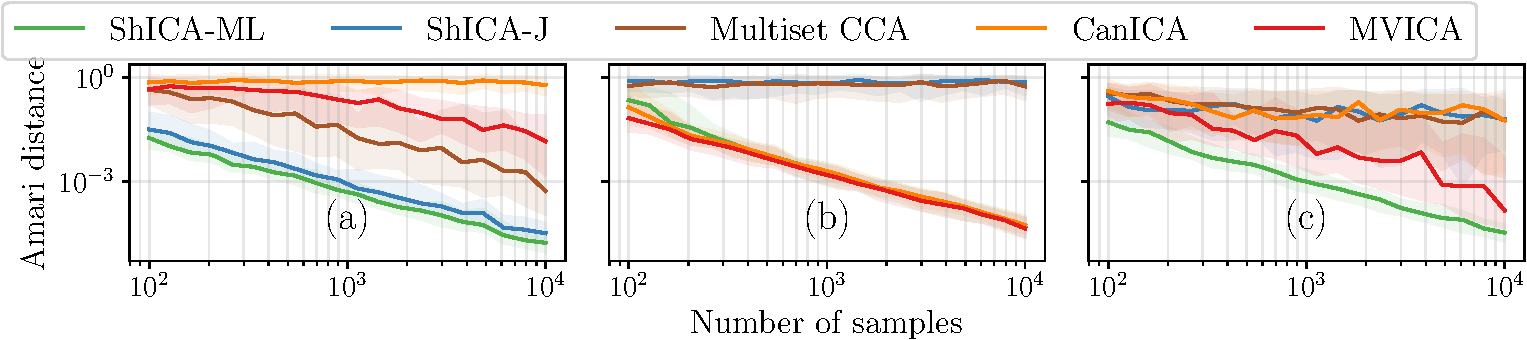
\includegraphics[width=0.9\textwidth]{./figures/amvica/identifiability.pdf}
  \vspace{-1em}
  \caption{\textbf{Separation performance}: Algorithms are fit on data following model~\ref{eq:model} \textbf{(a)} Gaussian components with noise diversity \textbf{(b)} Non-Gaussian components without noise diversity \textbf{(c)} Half of the components are Gaussian with noise diversity, the other half is non-Gaussian without noise diversity. 
  %\aapo{[It would be nice to have labels a,b,c but this is not critical.]}
  %\Alex{Make the legend fit on one line and rename Multiset CCA to Multiset CCA to be consistent with the text (or update text). Also you should be able to reduce a tiny bit the height of the axes plots.}
  }
  \label{exp:rotation}
  \vspace{-1.5em}
\end{figure}
When all components are Gaussian (Fig.~\ref{exp:rotation}~(a)), CanICA cannot separate the components at all. In contrast ShICA-J, ShICA-ML and Multiset CCA are able to separate them, but Multiset CCA needs many more samples to reach the same Amari distance as ShICA-J or ShICA-ML, which shows that correcting for the rotation due to sampling noise improves the results. Looking at error bars, we also see that the performance of Multiset CCA varies quite a lot with the random seeds: this shows that depending on the sampling noise, the rotation can be very different from identity.
When none of the components are Gaussian (Fig.~\ref{exp:rotation}~(b)), only CanICA and ShICA-ML are able to separate the components, as other methods do not make use of non-Gaussianity.
Finally, in the hybrid case (Fig.~\ref{exp:rotation}~(c)), only ShICA-ML is able to separate the components as it is the only method that can make use of both non-Gaussianity and noise diversity. Additional experiments illustrating the separation powers of algorithms are available in Appendix~\ref{app:separation}.
%

\vspace{-1.5em}
\subsection{Computation time}
\begin{wrapfigure}{l}{.47\textwidth}
    \centering
    \vspace{-1em}
    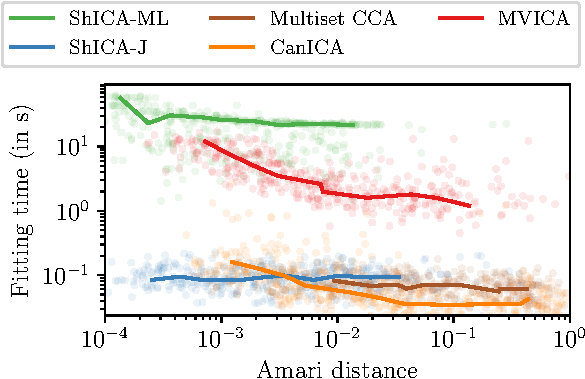
\includegraphics[width=.99\linewidth]{./figures/amvica/synthetic_gaussian_timings.pdf}
    \caption{\textbf{Computation time: } Algorithms are fit on data generated from model~\eqref{eq:model} with a super-Gaussian density. For different values of the number of samples, we plot the Amari distance and the fitting time. Thick lines link median values across seeds.}
    \label{exp:syn_timings}
\end{wrapfigure}
We generate components using a slightly super Gaussian density: $s_j = d(x)$ with $d(x) = x |x|^{0.2}$ and $x \sim \mathcal{N}(0, 1)$. We vary the number of samples $n$ between $10^2$ and $10^4$. We compute the mean Amari distance across subjects and record the computation time. The experiment is repeated $40$ times. We plot the Amari distance as a function of the computation time in Fig~\ref{exp:syn_timings}. Each point corresponds to the Amari distance/computation time for a given number of samples and a given seed. We then consider for a given number of samples, the median Amari distance and computation time across seeds and plot them in the form of a thick line.  From Fig~\ref{exp:syn_timings}, we see that ShICA-J is the method of choice when speed is a concern while ShICA-ML yields the best performance in terms of Amari distance at the cost of an increased computation time. The thick lines for ShICA-J and Multiset CCA are quasi-flat, indicating that the number of samples does not have a strong impact on the fitting time as these methods only work with covariances. On the other hand CanICA or MultiviewICA computation time is more sensitive to the number of samples.
%


%\pierre{fig might have a smaller legend: 3 cols, smaller fonts}


\paragraph{Robustness w.r.t intra-subject variability in MEG}
\begin{wrapfigure}{l}{.47\textwidth}
\vspace{-1.7em}
  \centering
  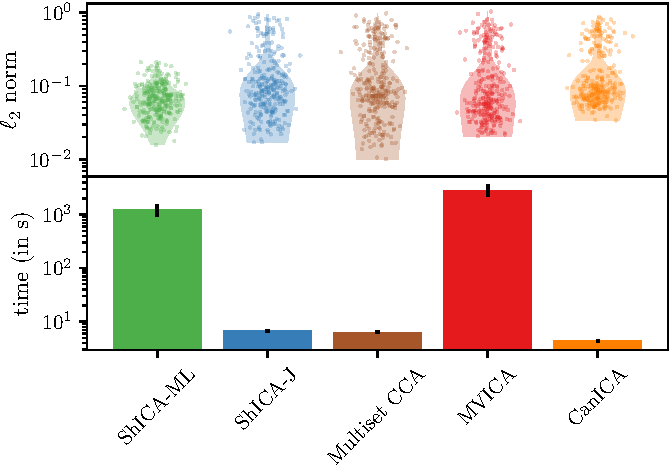
\includegraphics[width=.95\linewidth]{./figures/amvica/inter_subject_stability.pdf}
  \vspace{-0.5em}
  \caption{\textbf{Robustness w.r.t intra-subject variability in MEG}:
    (\textbf{top}) $\ell_2$ distance between shared components corresponding to the same stimuli in different trials.  (\textbf{bottom}) Fitting time.
    %\Alex{Should be $\ell_2$ in ylabel not L2}
}
\label{fig:eeg_intragroup_variability}
\vspace{-1em}
\end{wrapfigure}
In the following experiments we consider the Cam-CAN
dataset~\cite{taylor2017cambridge}. We use the magnetometer data from the MEG of $m=100$ subjects chosen randomly among 496.
% 
Each subject is repeatedly presented three audio-visual stimuli. 
% 
For each stimulus, we divide the trials into two sets and within each set, %Aapo: "sets"
the MEG signal is averaged across trials to isolate the evoked response. This
procedure yields 6 chunks of individual data (2 per stimulus).
%
% The 6 chunks of data are concatenated in the time direction and ICA algorithms
% are applied separately to extract $k=10$ shared components that we plot in
% appendix~\ref{megcomponents} and localize in appendix~\ref{megcomponentslocal}.
%
We study the similarity between shared components corresponding to repetitions of the same stimulus. This gives a measure of robustness of each ICA algorithm with respect
to intra-subject variability.
Data are first reduced using a subject-specific PCA with $p=10$ components. Algorithms are run 10 times with different seeds on the 6 chunks of data,
and shared components are extracted.
%
When two chunks of data correspond to repetitions of the same stimulus they should yield similar
components.
%
For each component and for each stimulus, we therefore measure the $\ell_2$
distance between the two repetitions of the stimulus.
 This yields $300$ distances per algorithm that are
plotted on Fig~\ref{fig:eeg_intragroup_variability}.

The components recovered by ShICA-ML have a much lower variability than other approaches. The performance of ShICA-J is competitive with Multiview ICA while being much faster to fit. Multiset CCA yields satisfying results compared with ShICA-J. However we see that the number of components that do not match at all across trials is greater in Multiset CCA.
    %\bt{Muliview ICA appears only now ?} \aapo{[Actually, multiset CCA looks just as good as ShICA-J?, comments?.]}
Additional experiments on MEG data are available in Appendix~\ref{app:phantom}.
% The difference between AVICA and other approaches can be quantified via a
% statistical t-test on the difference of log distances. It
% gives the p-values $4.57 \times 10^{-4}$, $5.93 \times 10^{-4}$ and $2.37
% \times 10^{-9}$ w.r.t.
% MVICA, PermICA and ConcatICA respectively.
\vspace{-1em}
\paragraph{Reconstructing the BOLD signal of missing subjects}
\begin{wrapfigure}{l}{.42\textwidth}
\vspace{-0.5em}
  \centering
  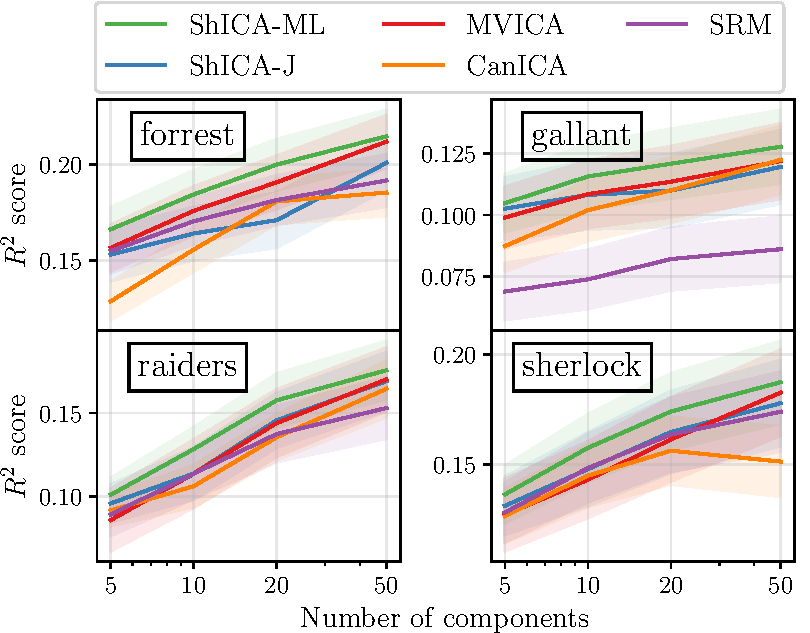
\includegraphics[width=0.99\linewidth]{./figures/amvica/reconstruction.pdf}
  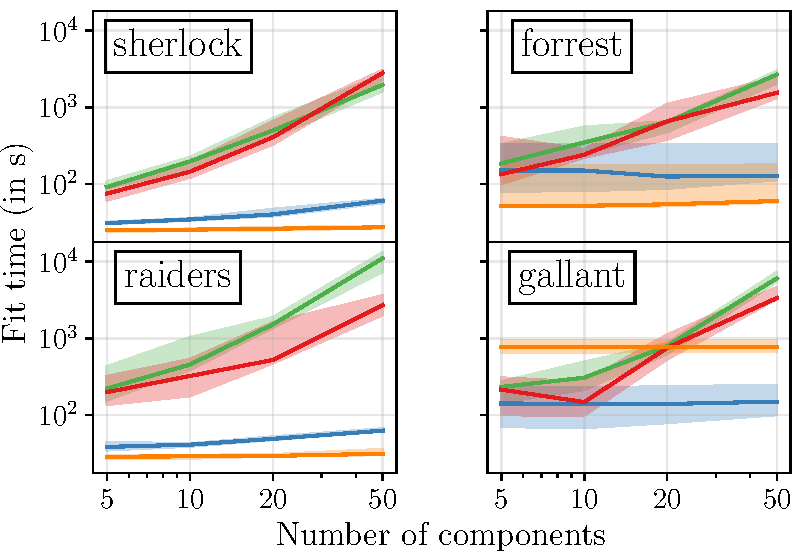
\includegraphics[width=0.99\linewidth]{./figures/amvica/reconstruction_timings.pdf}
  
  \caption{\textbf{Reconstructing the BOLD signal of
      missing subjects}. (\textbf{top}) Mean $R^2$ score between reconstructed data and true
    data. (\textbf{bottom}) Fitting time.
    %\Alex{ylabel should be $R^2$ not R2}
    }
  \label{fig:reconstruction}
\end{wrapfigure}
We reproduce the experimental pipeline of~\cite{richard2020modeling} to benchmark GroupICA methods using their ability to reconstruct fMRI data of a left-out subject.
%
The preprocessing involves a dimension reduction step performed using the shared response model~\cite{chen2015reduced}. Detailed preprocessing pipeline is described in Appendix~\ref{app:preprocessing}. We call an \emph{unmixing operator} the product of the dimension
reduction operator and an unmixing matrix and a \emph{mixing operator} its pseudoinverse. There is one unmixing operator and one mixing operator per view.
The unmixing operators are learned using all subjects
and $80\%$ of the runs. Then they are applied on the remaining $20\%$ of the runs using $80\%$
of the subjects yielding unmixed data from which shared components are extracted. We
then apply the mixing operator of the remaining $20\%$ subjects on the shared components to reconstruct their data.
%
Reconstruction accuracy is measured via the coefficient of determination, \aka
$R^2$ score, that
yields for each voxel the relative discrepancy between the true time course and the predicted one.
% :
% $R^2(\hat{\zb}, \zb) = 1 - \frac{\sum_{t=1}^n (z_t - \hat{z_t})^2}{\sum_{t=1}^n
%   (z_t - \bar{z})^2}$
% where $\bar{z} = \frac1n \sum_{t=1}^n z_t$ is the empirical mean of $\zb$.
%
For each compared algorithm, the experiment is run 25 times with different seeds to obtain error bars. We report the mean $R^2$ score across voxels in a region of interest (see Appendix~\ref{app:preprocessing} for details)
 and display the results in Fig~\ref{fig:reconstruction}. The error bars represent a $95\%$ confidence interval.
The chance level is given by the $R^2$ score of an algorithm that samples the coefficients of its unmixing matrices and dimension reduction operators from a standardized Gaussian. The median chance level is below $10^{-3}$ on all datasets. 
ShICA-ML yields the best $R^2$ score in all datasets and for any number of components. ShICA-J yields competitive results with respect to Multiview ICA while being much faster to fit. A popular benchmark especially in the SRM community is the time-segment matching experiment~\cite{chen2015reduced}: we include such experiments in Appendix~\ref{app:timesegment}.

% AVICA exhibits a small improvement on sherlock and raiders datasets that is
% consistent for different numbers of components (i.e. numbers of components) and competitive results on clips and forrest datasets.

% 

%\pierre{right plot is hard to read, too wide. Lots of space to gain here}

\section{Conclusion, Future work and Societal impact}
We introduced the ShICA model as a principled unifying solution to the problems of shared response modelling and GroupICA. ShICA is able to use both the diversity of Gaussian variances and non-Gaussianity for optimal estimation. We presented two algorithms to fit the model: ShICA-J, a fast algorithm that uses noise diversity, and ShICA-ML, a maximum likelihood approach that can separate Gaussian and non-Gaussian components. ShICA algorithms come with principled procedures for shared components estimation, as well as adaptation and estimation of noise levels in each view (subject) and component. On simulated data, ShICA clearly outperforms all competing methods in terms of the trade-off between statistical accuracy and computation time. On brain imaging data, ShICA gives more stable decompositions for comparable computation times, and more accurately predicts the data of one subject from the data of other subjects, making it a good candidate to perform transfer learning. ShICA inherits the ethical questions linked to its field of application. However, as it involves linear transforms, decisions based on its output are easier to interpret. This work can help in brain disease diagnosis and reduce their human and societal burden.

% \section{A fast two-step approach for MIFA}

% While maximum-likelihood approaches possess several important statistical properties that make them attractive, a major drawback is the slowness of the algorithms. 
% %
% These method also require the likelihood to be well defined, and prevents dimension reduction without a more complicated model: for the likelihood to be well defined, we must assume that $A_i$ is square, invertible.
% Instead, we propose a two steps ad-hoc method, based on the following observations that were used for proving identifiability:
% \begin{itemize}
%     \item The knowledge of the empirical covariances $C_{ij}$ for $i\neq j$ allows to recover the mixing matrices $A_i$ up to a global rotation matrix.
%     \item Then, the knowledge of the ``diagonal'' terms $C_{ii}$ allows to eliminate this indeterminacy
% \end{itemize}
% These observations lead to the following two step approach
% \paragraph{Dimension reduction and global estimation}
% We first estimate jointly all the mixing matrices up to a global rotation by minimizing the criterion $\mathcal{L}(A_1, \dots, A_m) = \sum_{i \neq j} \|A_iA_j^{\top} - C_{ij}\|_F^2$.
% Since this cost function is quadratic with respect to each $A_i$, it is easily minimized w.r.t. one of the variable when all others are fixed:

% $$
% \arg\min_{A_i}\mathcal{L}(A_1\dots, A_m) = \left(\sum_{j\neq i} C_{ij}A_j\right)\left(\sum_{j\neq i}(A_j)^{\top}A_j\right)^{-1}
% $$
% Importantly, this formula also holds when the problem is over-determined, i.e. when $A_i\in \mathbb{R}^{p\times d}$ with $d < p$.
% We can then loop over all coordinates several times to obtain a block-coordinate descent algorithm. Each iteration of the algorithm is guaranteed to decrease the loss function. 
% The following lemma shows that minimizing the cost function leads to estimates of the true mixing matrices up to a global indeterminacy.
% \begin{prop}
% Assume that for $i\neq j$, $C_{ij}= B_iB_j^{\top}$ for some matrices $(B_i)_{i=1}^m\in\mathbb{R}^{p\times d}$ with $d< p$. Then, $\mathcal{L}(A_1, \dots, A_m) = 0$ if and only if there exists $U\in\mathcal{O}_d$ such that $A_i = B_i U$ for all $i$.
% \end{prop}
% {\textcolor{red}{Can we say anything about the algorithm ?  does it reach a local / global minimum?}}
% As a consequence, minimizing the previous criterion allows to reduce the dimension of the data. Importantly, since the problem is non-convex, we have no guarantee that the proposed algorithm reaches a global optimum. In practice, we found the proposed method to be robust.
% The last part of the procedure estimates the global rotation $U$ using joint diagonalization.
% \paragraph{Estimation of the global rotation by joint-diagonalization}
% We use the following property to estimation the global rotation.
% \begin{prop} Assume that $C_{ii} = B_i(I_d + D_i)B_i^{\top}$ with $D_i$ a diagonal matrix with positive entries. Let $U$ an  orthogonal matrix, and $A_i = B_i U$, and $K_i = A_i^{-1}C_{ii}A_i^{-\top}$. Then, $U$ is a joint-diagonalizer of the set $K_i$, i.e. the matrices $U^{\top}K_i U$ are all diagonal.
% \end{prop}
% Therefore, letting $A_i$ the outputs of the previous algorithms, we form the matrices $K_i$, and estimate the global rotation $U$ by joint-diagonalization of the $K_i$. The estimate of the mixing matrix is then $A_i U^{\top}$.